\documentclass[tikz,dvipsnames]{standalone}
\usepackage{amsmath}

\begin{document}

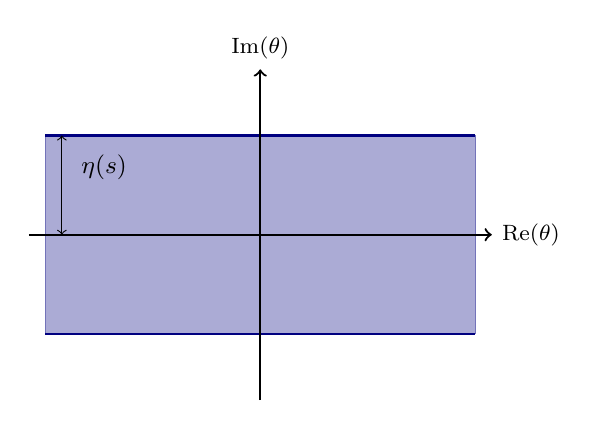
\begin{tikzpicture}[scale=0.84]
        
    \node (a) at (-3.25,1.5) {};
    \node (b) at (3.25,1.5) {};
    \node (c) at (-3.25,-1.5) {};
    \node (d) at (3.25,-1.5) {};
    \filldraw[NavyBlue!55,fill opacity=0.6] (a.center)--(b.center)--(d.center)--(c.center)--cycle;
    \draw[thick,NavyBlue] (a.center)--(b.center);
    \draw[thick,NavyBlue] (c.center)--(d.center);
    \draw[->,thick] (-3.5,0)--(3.5,0) node[right]{\footnotesize{$\operatorname{Re}(\theta)$}};
    \draw[->,thick] (0,-2.5)--(0,2.5) node[above]{\footnotesize{$\operatorname{Im}(\theta)$}};
    \node[label=below right:\small{$\eta(s)$}] (e) at (-3,1.5) {};
    \node (f) at (-3,0) {};
    \draw[->] (e.center)--(f.center);
    \draw[->] (f.center)--(e.center);
    \end{tikzpicture}

\end{document}